\chapter{Introduction}
% Change page numbers back to Arabic numerals and reset the page count
\renewcommand{\thepage}{\arabic{page}}
\setcounter{page}{1}

As shown in Figure \ref{intro}, two robots perform a competition in this project. Two robots chase each other and try to hit the opponent with laser, which are controlled via intelligent algorithms. This report mainly introduces the algorithms for image processing and robot control.

\begin{figure}[thb]
    \centering
    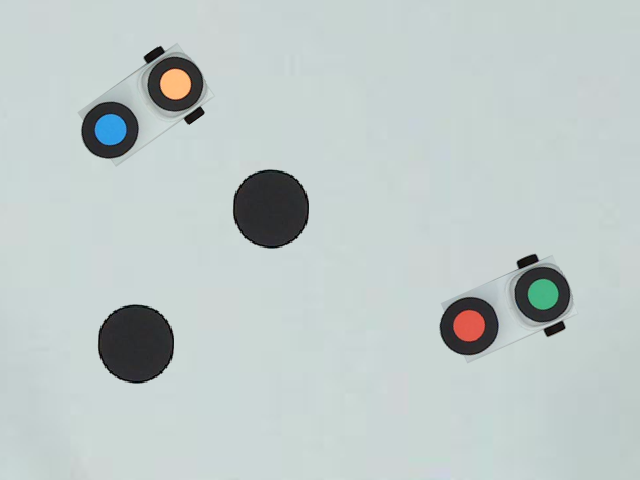
\includegraphics[width=0.5\textwidth]{images/intro.png}
    \caption[Overview of the project]{Overview of the project.}
    \label{intro}
\end{figure}

\section{Modelling of the Robot 1}\label{robot_modelling}

There is no wheel slipping, 

\begin{figure}[thb]
    \centering
    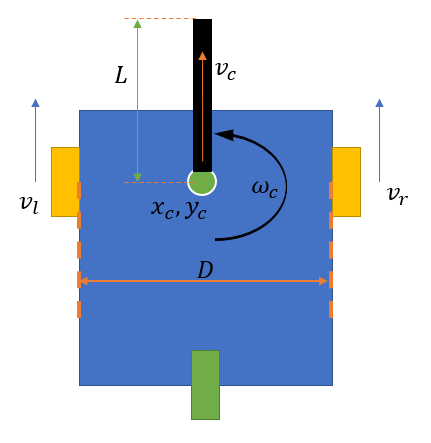
\includegraphics[width=0.5\textwidth]{images/vehicle_model.png}
    \caption[vehicle model]{vehicle model.}\label{intro}
\end{figure}

$$ v_r = \omega_r R $$


\begin{figure}[thb]
    \centering
    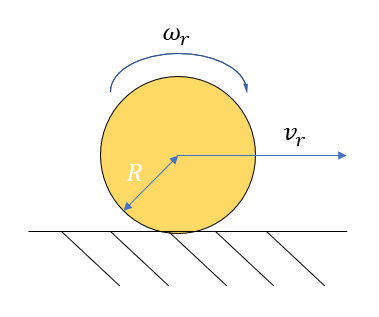
\includegraphics[width=0.6\textwidth]{images/wheel_model.png}
    \caption[wheel model]{wheel model.}\label{intro}
\end{figure}
Where $v_r$ is the linear velocity, $R$ is the radius of wheel, and $\omega_r$ is the angular velocity.

$x_c$ and $y_c$ is the coordinate of the vehicle centre. $\theta$ is the direction of vehicle. $D$ is the distance bewteen two wheels. The geometry model of this vehicle is shown below:

$$ v_c = (v_r+v_l)/2 $$
$$ \omega_c = ( v_r - v_l ) / D $$
$$ \dot{\theta_c} = \omega_c = ( v_r - v_l ) / D $$



